\documentclass[twocolumn]{article} % -[...]
\usepackage[top=.5in, bottom=.5in, left=.75in, right=.75in]{geometry} % -[...]
\usepackage{hyperref}
\usepackage{graphicx}
\usepackage{subcaption}
\usepackage{amsthm,amssymb,amsmath}
\usepackage{moreverb}
\usepackage{blkarray, bigstrut}
\usepackage{tikz}
\usepackage{arabtex}
\usepackage{utf8}
\title{A sample \LaTeX\ document}
\author{
vSpades \\ \url{vegaspades@gmail.com}
\and % -\and
foo bar \\ \url{foo@bar.zone}
}
\date{} % to stop this-date.
\begin{document}
\setcode{utf8}
\maketitle % to stop a whole-page.
\begin{abstract}
This article demonstrate a sample paper which produced by \LaTeX.
\end{abstract}
\section{Introduction}\indent
This is the output of a sample \textit{.tex} document in PDF. One could
investigate through the codes, commands and comments to find out how each of
them parts have been done.

While this simple paper recaps only the most essential features, there are
plenty of resources \cite{web:1}\cite{web:2}\cite{web:3} that walk us through
much fancier stuffs that could be done by \LaTeX.
\section{Reshaping Text}
The following is a short list of common formats to reshape texts:
\begin{enumerate}
\item This is a \textbf{bold phrase}.
\item This is an \textit{italic phrase}.
	\begin{enumerate}
	\item sub-item-a
	\item sub-item-b
	\end{enumerate}
\item This one is \underline{underlined}.
\end{enumerate}
To avoid ``\emph{Plagiarism}'' please cite lines. Using quotes, references, ...
are various methods to do such. Plenty types of sources (Website, Article, Book
Chapter, ...) \cite{web:4} might be referred to using \textit{BibTeX}.
\section{Figures and Images}
To display an image or a photo we may use \textit{graphicx} package. Figure
\ref{fig:1} shows one single photo.
\begin{figure}[bh!]
\centering
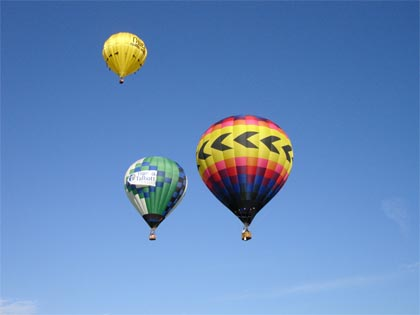
\includegraphics[width=.5\linewidth]{asset/img1.jpeg}
\caption{hot air balloons --
\url{https://www.dike.lib.ia.us/images/sample-1.jpg/image_view_fullscreen}}
\label{fig:1}
\end{figure}

It is also possible to do that with multiple images (\ref{fig:2}) and
(\ref{fig:3}) side by side, using \textit{subcaption} package.
\begin{figure}[h!]
\centering
\begin{subfigure}[b]{0.4\linewidth}
\includegraphics[width=\linewidth]{example-image-a}
\caption{sample-image-a}
\label{fig:2}
\end{subfigure}
\begin{subfigure}[b]{0.4\linewidth}
\includegraphics[width=\linewidth]{example-image-b}
\caption{sample-image-b}
\label{fig:3}
\end{subfigure}
\end{figure}

Both of them images generated with \LaTeX\ commands. We might as well build more
advanced drawings using other extra packages. On top of that, there are always
external softwares that could produce drawings in PDF output. We elaborate on
that in section \ref{sec:1}.
\section{Math Expressions}
An \textit{inline} formula like, Einstein's Equation: $E = mc^2$. and then
\textit{multiple-line} equations:
\begin{equation*}
sin^2x + cos^2x = \frac{a^2 + b^2}{c^2}
\end{equation*}
\begin{equation*}
Pythagorean: a^2 + b^2 = c^2
\end{equation*}
\begin{equation*}
\Rightarrow sin^2x + cos^2x = 1
\end{equation*}
In addition, code scripts could be displayed \textit{as-it-is}:
\begin{verbatimtab}
// a "hello-word" example in C:
#include <stdio.h>
void main() {
	printf("hello, world!");
	printf("\n");
}
\end{verbatimtab}
\section{Diagrams}
\label{sec:1}
Scientific papers may include tables, matrices, graphs or other types of
diagrams to display some information. In this section we represent a table
\ref{tab:1} and a matrix \ref{tab:2} which is a specific form of a table. Figure
\ref{fig:4} demonstrates a graph (via \textit{Tikz}) represents the same
information.

\begin{table}[h!]
\begin{center}
% alignments: 1st column (l)eft, 2nd (c)enter and 3rd (r)ight,
% with vertical lines in between.
\begin{tabular}{l|c|r}
\textbf{who} & \textbf{likes} & \textbf{whom}\\
\hline
foo & 1 & bar\\
foo & 1 & baz\\
bar & 1 & foo\\
bar & 0 & baz\\
baz & 0 & foo\\
baz & 0 & bar\\
\end{tabular}
\end{center}
\caption{Friendship}
\label{tab:1}
\end{table}
% sample: b-mat & p-mat --
%\[
%\begin{pmatrix}
%	x_{11} & x_{12} & x_{13} & \dots & x_{1n} \\
%	x_{21} & x_{22} & x_{23} & \dots & x_{2n} \\
%	\hdotsfor{5} \\
%	x_{d1} & x_{d2} & x_{d3} & \dots & x_{dn}
%\end{pmatrix}
%=
%\begin{bmatrix}
%	x_{11} & x_{12} & x_{13} & \dots & x_{1n} \\
%	x_{21} & x_{22} & x_{23} & \dots & x_{2n} \\
%	\vdots & \vdots & \vdots & \ddots & \vdots \\
%	x_{d1} & x_{d2} & x_{d3} & \dots & x_{dn}
%\end{bmatrix}
%\]
\begin{table}[h!]
\begin{center}
%\centering
\begin{minipage}[!hbt]{.5\textwidth}
\[
A_{(Friendship)} =
\begin{blockarray}{cccc}
& foo & bar & baz \\
\begin{block}{c[ccc]}
foo & NA & 1 & 1 \\
bar & 1 & NA & 0 \\
baz & 0 & 0 & NA \\
\end{block}
\end{blockarray}
\]
\end{minipage}
\end{center}
\caption{Matrix of Friendship}
\label{tab:2}
\end{table}

\begin{figure}[bh!]
\centering
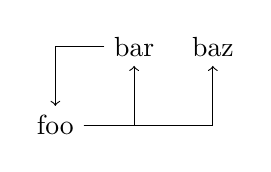
\begin{tikzpicture}[node distance=2cm]
% nodes
\node (A) at (0, 0) {foo};
\node (B) at (1, 1) {bar};
\node (C) at (2, 1) {baz};
% arrows
\draw[->, to path={-| (\tikztotarget)}]
(A) edge (B) (A) edge (C) (B) edge (A);
\end{tikzpicture}
\caption{Graph of Friendship by CTAN:Tikz}
\label{fig:4}
\end{figure}
There are more methods to draw graphs. The following compares two other ones.
\subsection{PyPI NetworkX}
NetworkX is a Python package to study complex and dynamic networks \cite{web:5}.
With only a few lines of codes \footnote{``.PY'' source-code is available inside
the same repo:sampleTeX/asset}, we could draw a decent graph (Figure
\ref{fig:5}).
\begin{figure}[bh!]
\centering
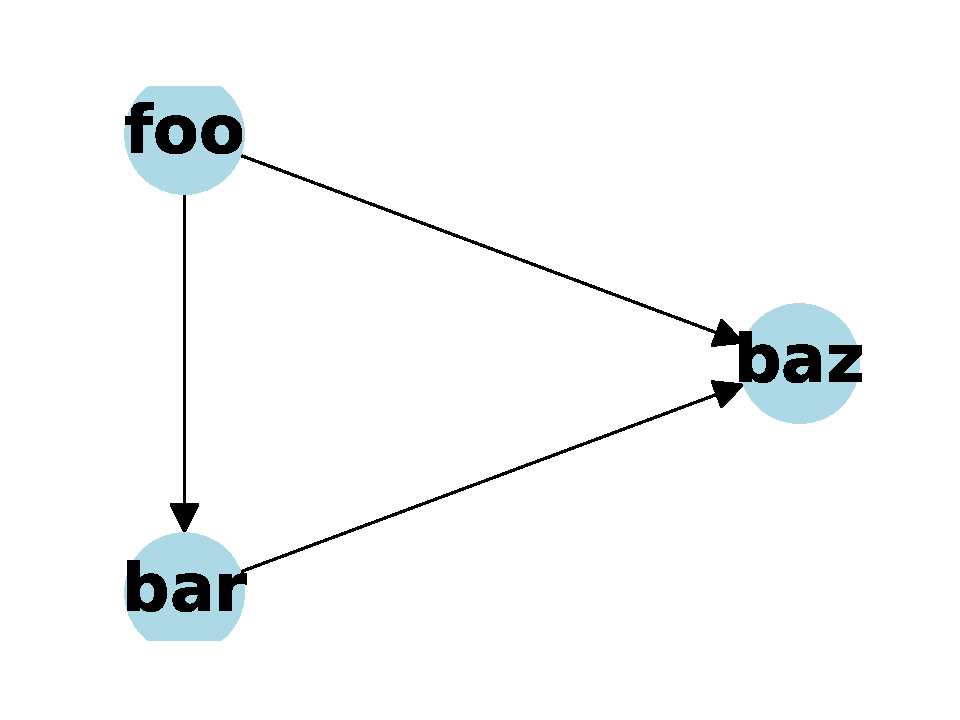
\includegraphics[width=.5\linewidth]{asset/nx_fig1.pdf}
\caption{Graph of Friendship by PyPI:NetworkX}
\label{fig:5}
\end{figure}
\subsection{LibreOffice Draw}
External Softwares could also become handy for this matter. Figure \ref{fig:6}
has been built \footnote{``.ODG'' draw-file is available inside the same
repo:sampleTeX/asset} by LibreOffice Draw \cite{web:6}.
\begin{figure}[bh!]
\centering
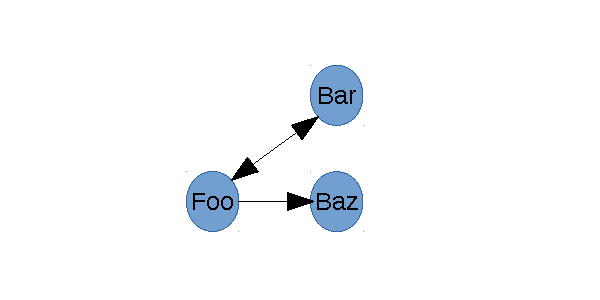
\includegraphics[width=.5\linewidth]{asset/draw_fig1.pdf}
\caption{Graph of Friendship by LibreOffice:Draw}
\label{fig:6}
\end{figure}
\section{Bilingual}
It is possible to drop some lines in non-ascii (UTF-8 like; Arabic, Persian,
...) among text. The following provides a combination of English and Arabic
\footnote {Extra Persian letters also supported.}. We need to distinguish
different language using
\begin{verbatim}
\begin{arabtext}
...
\end{arabtext}
\end{verbatim}.
\section*{Example}
Say Hello to
\begin{arabtext}
پارسی
\end{arabtext}
and back to English again.

Whereas the entire paper (or most parts of it) could be in Persian. In such
case, the\textit{``xepersian''} package is strongly recommended.
\footnote{``farsi.tex'' tex-document is available inside the same
repo:sampleTeX}
\section{Conclusion}
Summery of this article and explaining future works.
\bibliography{src}
\bibliographystyle{ieeetr}
\end{document}
%whatever, literally whatever comes after \end{document}, won't get interpreted.
%هر چی باشه
